%\documentclass[10pt,fleqn]{article}
%\documentclass[letterpaper,10pt,fleqn]{article}
\documentclass[twoside,twocolumn,10pt,fleqn]{article}
\usepackage[margin=1in,columnsep=20pt]{geometry}
\usepackage{amsmath}
\usepackage{amsthm}
\usepackage{amsfonts}
\usepackage{amssymb}
\renewcommand{\theequation}{\arabic{equation}}
\usepackage[ruled]{algorithm2e}
\usepackage{tikz}
\usepackage{hyperref}

\newcommand*{\ABSTRACT}{}

\title{A Byzantine Fault-tolerant KV Store for Decentralized PKI and
  Blockchain\\(Extended Abstract)\footnotemark[1]}

\author{%
  \textsc{Ryuji Ishiguro}
}
\date{\today}

\usepackage{titling} % Customizing the title section
\usepackage{abstract} % Allows abstract customization
\renewcommand{\maketitlehookd}{%
  \begin{center}
    \url{https://github.com/yahoo/bftkv}
  \end{center}
  \begin{abstract}
  \noindent
  Most distributed key-value stores are tolerant to only benign
  failure, which makes it difficult to run the system in an insecure
  environment (i.e., the Internet) as single point of failure could
  compromise the whole system.  Such systems not only are vulnerable to
  malicious attacks, but also need to rely on centralized authorities to
  protect data integrity.
  We developed a distributed key-value store that is tolerant
  to Byzantine faults, keeping it in mind to run the system over the
  public Internet without any central
  authorities.  While data integrity is secured among distributed
  nodes, all transactions are transparent to anyone.
  The system provides not only a robust key-value store but also data
  secrecy and distributed signing features with a threshold
  cryptosystem. Integrating encryption and signature schemes with
  a Byzantine fault-tolerant protocol is much more robust than using
  separated KMS and PKI with an ordinary distributed key-value store,
  as it maximizes a benefit of distributed systems which fit very well
  with threshold cryptography. There is no single point of failure in
  the system.
  The system by itself is useful as a secure key-value store, but those
  properties such as Byzantine fault-tolerance, transparency,
  distributed global storage and threshold cryptosystem can make the
  system an ideal building block for blockchain technologies.
\end{abstract}

}

\begin{document}

\maketitle

\footnotetext[1]{The full paper is available from the github
  repository. \url{https://github.com/yahoo/bftkv/tree/master/docs/bftkv.pdf}}

\section{Introduction}
How to reach a consensus with Byzantine type failure is the main
problem of blockchain technologies. Bitcoin blockchain uses PoW (Proof
of Work) with incentives \cite{bitcoin}. The majority of public
blockchain (or permission-less blockchain) systems have the same type
of consensus mechanism. Another way to establish a consensus is to use
BFT (Byzantine Fault-Tolerant) protocols, which is a major mechanism
for local/enterprise blockchain (or permissioned system). Some PoS
(Proof of Stake) type blockchain technologies use BFT as well to avoid
the mining process.

The proposed system is based on the Byzantine quorum system introduced
by Malhi and Reiter \cite{Delhi:1}, and adopts a BFT protocol proposed
by the same authors \cite{Delhi:2}. We construct a $b$-masking quorum
system based on the WoT (Web of Trust) graph. We also introduce quorum
certificates combined with a threshold authentication scheme to
protect data from unauthorized mutation. Unlike a centralized PKI such
as X.509, quorum certificates are verified collectively with other
quorum members that are chosen with a dynamic graph constructed
independently at each node. With the strong authentication scheme
backed by a threshold cryptosystem and flexible certificate mechanism,
the system allows anyone to join / leave the network freely without
any authorization process while it is immune from sybil attacks.

Another key aspect of blockchain technologies is the global
distributed ledger. Bitcoin blockchain uses hash chain -- transactions
in a specific period are all hashed together with the hash value of
the previous block. All bitcoin nodes maintain the same view of the
hash chain.
The proposed system uses a distributed key-value store with the TOFU
(Trust on First Use) policy, that is, the first use of a key locks out
others from mutating the value associated with the key. Only the
user who has written the key-value first will posses the right to
update the value. Also it supports WRITE ONCE permission which
guarantees that once a value is written it will never be modified in
any way. This special permission will be preferable for applications
like the global ledger which must be tamper-proof.
The system does not guarantee absolute consistency. Also the order of
transactions for different keys does not matter. The system does not
even provide eventual consistency among individual nodes. Instead, it
has a property such that: $READ(Q_1, x) = READ(Q_2, x), \forall Q_1,
Q_2 \in QS$, that is, the consistency is established collectively with
a quorum system ($QS$).

Smart contracts play an important role in some blockchain technologies
such as Ethereum and Hyperledger Fabric. As the proposed system is a simple
key-value store, it does not provide a platform for smart contracts at
the moment. Also, the system itself does not provide any incentive
mechanism to discourage nodes to do malicious actions, or to encourage
to participate the consensus process. The system has a robust
revocation scheme but it does not answer for a question like why would
one want to run a node? Although all transactions keep a proof of good
or bad actions for each node therefore it will be straightforward to
map it to economic incenstives and penalties, we defer fintech
discussions to an application layer.


\section{Methodology}
This section describes quorum systems based on the WoT graph, which
are the main building blocks for our BFT protocols. Protocols are
always between a client and a quorum. Every message must be signed by
a set of special nodes called {\em Quorum Cliques}, and stored in
another quorum called {\em KV quorum}. To write a key-value pair the
client performs the three step process:
\ifdefined\ABSTRACT
\footnote{Detailed protocols are described in the full paper.}
\fi
\begin{enumerate}
\item Collect timestamps from a quorum and choose the latest one,
\item Request to sign the message to a quorum in the {\em Quorum Cliques},
\item Write the signed message to a {\em KV quorum}.
\end{enumerate}
To read a key-value pair, the client performs the following process:
\begin{enumerate}
\item Collect key-value pairs from a {\em KV quorum}
\item Choose the latest one
\end{enumerate}
\ifdefined\ABSTRACT
\else
See the section \ref{Protocols} below for details.
\fi

In order to complete the system, authentication and signature schemes
based on a threshold cryptosystem are introduced in this section as
well.

\subsection{Quorum Cliques}
We follow the faulty clients (or dishonest writers) scenario described
in ``Byzantine Quorum Systems'' \cite{Delhi:1,Delhi:2}, which uses
signed messages with $b$-masking quorum systems to avoid equivocation.
\footnote{Aka double-spending in the blockchain world.}
In our system, such quorum system is constructed from maximal cliques
in the WoT graph.

If the graph $G$ contains some cliques and the starting node $s$ has
outdegree edges to the cliques within the $L$ distrance, i.e.,
\[
\exists (s, u) \in G.E, s.t., u \in QC \text{ and } dist(s, u) \le L \\
\]
where $QC$ is quorum cliques obtained by the algorithm {\sf GetQC}
\ref{GetQC},
it will construct a quorum to sign messages. Note that the quorum
depends on only the graph $G$. There are no other configuration data
or anything.
Such graph is constructed from the quorum certificates. 

\subsubsection*{Quorum Certificates}
Quorum certificates represent the proof of trustworthy. Each node
keeps its own quorum certificate along with the private key. 
A quorum certifiate consists of:
\begin{itemize}
\item a unique ID
\item a public key
\item a self signed signature over the ID and public key
\item a set of signatures signed by Quorum Cliques
\end{itemize}
When a node ($n_1$) is signed by another node ($n_2$) an edge is added
to the WoT graph, i.e., $G.E = G.E \cup \{(n_2, n_1)\}$.

The quorum certificate not only constructs the graph but also gives
permissions to clients to mutate the value.
Every {\sf write} request includes the client's quorum certificate
along with the self signed signature over the variable, timestamp and
value which we denote $\langle x, t, v \rangle$.
Each member of $QC$ verifies the signature and the quorum
certificate before it sends back the signed message. See algorithms
{\sf VerifyCollectiveSignatures} \ref{VerifyCollectiveSignatures} and
{\sf CheckQuorumCert} \ref{CheckQuorumCert}.

\subsubsection*{Sybil Attack}
When a node is compromised the node can try to make its own cliques
with made-up colluding nodes to outnumber the honest nodes. By the
algorithm {\sf GetQC} \ref{GetQC} which is used to verify the quorum
certificates and the collective signatures, a node cannot be a
member of more than one cliques, which means the compromised node has
to sever the trust links to other nodes itself to make links with the
colluding nodes, otherwise the clique can no longer be a member of a
quorum. If such a faulty clique disagrees with other cliques a
consensus will be no longer established until clients exclude the
compromised nodes.

\subsection{Key-value Store}
Once data is signed by quorum cliques it can be sent to other nodes
that are not necessarily members of the cliques. Such nodes can form
another quorum system and we call it {\em KV quorum}. The main purpose
of this quorum system is to make sure that clients can retrieve the
latest key-value. We no longer need the $b$-masking quorum as all
messages are signed by quorum cliques which have already handled the
faulty client case. {\em KV quorum} handles only $f$ benign faulty
nodes. The {\sf read} process writes back the latest message to nodes
that keeps old values:
\begin{enumerate}
\item The client collects $f + 1$ responses and chooses one which
  has the latest timestamp.
\item If some servers return an old value or {\em
    nil} the client will write back the latest value to those servers.
\end{enumerate}
\ifdefined\ABSTRACT
\else
See ~\ref{rw} for the actual protocols.
\fi
For load balancing, {\em KV quorum} is typically chosen from $U
\setminus\; QC$.

Each member of {\em KV quorum} must check equivocation and the
permission of mutation (TOFU), when it receives the signed
transaction.

\subsubsection*{Equivocation Check / Revocation}
Revocation is the only way to keep the system sound in the long
run. Keeping the number of faulty nodes within the quorum threshold is
the key to the soundness of the system.

Each node severs the trust link independently without consulting
others when it detects a node that has signed both $\langle x,t,v
\rangle$ and $\langle x,t,v' \rangle$ s.t.  $v \neq v'$. Also servers
revoke clients when it detects a client signing different values with
the same timestamp as well. Once a node is revoked, it will be
excluded from the WoT graph forever and there is no way to restore it.
See algorithm {\sf CheckEquivocation} \ref {CheckEquivocation} for
the equivocation check.

\subsubsection*{TOFU Policy}
The system enforces the TOFU policy on every write request. If the
slot is empty each node in the KV quorum will simply store the
data. If the slot already has data, the node first retrieves the
latest data and check if the signer is the same as the one of the
requested data.  See {\sf CheckTOFU} \ref{CheckTOFU} for the
algorithm to check the TOFU policy.

\subsection{Threshold Password Authentication ($\mathcal{TPA}$)}
\label{auth}
The quorum system based on the WoT graph guarantees data
integrity. The TOFU policy with the quorum certificate prevents
unauthorized mutations. The collective signatures make it possible to
check equivocation. All those functions rely on the digital signature
scheme therefore managing the signing key is significantly
important for this system. We use a threshold password authentication
($\mathcal{TPA}$) for:
\begin{itemize}
\item enrolling nodes to the system
\item recovering from a key-loss situation
\item sharing an ID with multiple devices
\item data secrecy (roaming encryption)
\end{itemize}
$\mathcal{TPA}$ is immune from offline dictionary attacks (as long as
the number of compromised servers is less than the threshold). The
authentication protocol is similar to \cite{ford} by Ford and Kaliski,
but the shared secret is calculated by Shamir's Secret Sharing (SSS)
\cite{shamir}.\\

To set up the {\em shares} the client generates a random polynomial
for $(t, n)$ SSS over a prime field $\mathbb{Z}_q$, s.t.,
\[
  f(x) = \sum_{i=0}^{t-1}a_ix^i \bmod q
\]
then calculates $n=|Q|$ pairs $(i,f(i)), i = 1..n$. The shared secret
is $S = f(0)$. Each {\em share} will be $\langle i, y_i, v_i, t_i
\rangle$,
where:
\begin{align*}
  y_i &= f(i) \\
  v_i &= g_{\pi}^{Ss_i} \bmod p \\
  s_i &= \text{OS2I}(h(password, t_i)) \\
  g_{\pi} &= \pi^2 \bmod p \\
  \pi &= \text{OS2I}(h(password))
\end{align*}
$p$ and $q$ are prime numbers such that $p = 2q + 1$ (i.e., $p$ is a
safe prime). $t_i$ is a salt. The random polynomial must be generated
randomly for each password.\\

To get a password authenticated:
\begin{enumerate}
\item The client generates a random number
  $a \xleftarrow{\mathcal{R}} \mathbb{Z}_q$
  and calculates $X$ from the password:
  \[
    X = g_{\pi}^a \bmod p
  \]
  then broadcast it to a quorum $Q$.

\item Each quorum member returns:
  \[
    Y_i = X^{y_i} \bmod p
  \]
  with the salt $t_i$.

\item The client collects $t$ responses from the quorum ($\mathcal{T}
  \subseteq Q$), and
  calculates:
  \[
    G_S = \prod_{j \in \mathcal{T}}Y_i^{\lambda_j} \bmod p
  \]
  where each $\lambda_j$ is the lagrange interporate:
  \[
    \lambda_j = \prod_{l \in \mathcal{T} \setminus \{j\}}
    i_l / (i_l - i_j) \bmod q.
  \]
  Then, generate another random number $a' \xleftarrow{\mathcal{R}}
  \mathbb{Z}_q$ and for each server $i \in \mathcal{T}$, calculate and
  send back:
  \[
    X_i = G_S^{s_ia'} \bmod p
  \]
  where
  \[
    s_i = h(password, t_i)
  \]

\item Each quorum member($\in \mathcal{T}$) generates a random exponent
  $b_i \xleftarrow{\mathcal{R}} \mathbb{Z}_q$
  for a DH session key:
  \[ K_i = X_i^{b_i} \bmod p \]
  and encrypts the proof ($P_i = Sig_i(\centerdot)$):
  \[
    Z_i = E_{h(K_i)}(P_i, X || Y_i)
  \]
  then sends it back to the client with
  \[
    B_i = v_i^{b_i} \bmod p.
  \]

\item The client decrypts $Z_i$ with
  \[
    K_i = B_i^{aa'} \bmod p
  \]
  and gets:
  \[
    (P_i, N) = D_{h(K_i)}(Z_i).
  \]
  Check if $N = X||Y_i$ to make sure both parties have shared the
  session key correctly. 
\end{enumerate}
We use $\{P_i\}_{\{i \in \mathcal{T}\}}$ as the proof of
authentication which will be attached to protocol messages and checked
at each node during the {\sf read / write / register} protocols. The
signed data in each $P_i = Sig_i(\centerdot)$ depends on those
protocols.

\ifdefined\ABSTRACT
Here is a brief explanation of correctness
\footnote{See the full paper for a security analysis.}.
Assume $\{Y_i\}_{\{i \in \mathcal{T}\}}$ is correctly calculated,
$G_S$ will be:
\[
  G_S = \prod_{j \in \mathcal{T}}Y_i^{\lambda_j} = g_{\pi}^{a \sum_{j
      \in \mathcal{T}} f(j) \lambda_j} = (g_{\pi}^S)^a \bmod p
\]
and by raising $s_i = h(password, s_i)$ to $G_S$, we get:
\[
  X_i = G_S^{s_i} = (g_{\pi}^{Ss_i})^a \bmod p
\]
which must be the same as $v_i^a \bmod p$ for each $i \in
\mathcal{T}$ iff the correct password ($g_{\pi}$) is given at the
step 1. With each $B_i = v_i^{b_i} \bmod p$, the client and servers
share DH keys $K_i = g_{\pi}^{Ss_iab_i} \bmod p$.
\else
See Appendix \ref{tpa} for correctness and security analysis of
$\mathcal{TPA}$.
\fi

\subsubsection*{$\mathcal{TPA}$ for Enrollment}
$\mathcal{TPA}$ is used to enroll new nodes to the system so it can
recover from a key-loss situation and support multiple devices per
user.\\

\noindent
Enrollment:
\begin{enumerate}
\item Generate a unique ID and a key pair,
\item Send the certificate signing request to a quorum with the
  $\mathcal{TPA}$ {\em shares} to get a quorum certificate.
\end{enumerate}

\noindent
Key recovery / secondary key generation:
\begin{enumerate}
\item Generate a new key pair with the existing ID,
\item Do the password authentication and get a proof,
\item With the proof, send the new certificate to a quorum to get a new
  quorum certificate.
\end{enumerate}
\ifdefined\ABSTRACT
\else
See \ref{register} for the actual protocols.
\fi

\subsubsection*{$\mathcal{TPA}$ for Data Secrecy}
The system provides a roaming service to store and access encrypted
data. Users encrypt a value at a node then send the encrypted value
to a quorum. They can decrypt the value at any node with the
password. The password is stored along with $\langle x, t, v \rangle$.
The encryption key is $h(g_{\pi}^S)$. $S$ (and the random polynomial
as well) has to be randomly generated everytime the data is encrypted
at a client.

To decrypt the data the user specifies the variable $x$ along with the
password then the client starts the threshold password authentication
process first to get the proof. With the proof the client proceeds the
{\sf read} process and decrypts the value with the above key.

With this roaming scheme, BFTKV can be a secure vault that is not only
fault-tolerant for high availability but immune to single point of
failures. The same kv storage can be used to keep both public / private
keys without relying on a separated KMS.

\subsection{Distributed Signing}
Some crypto-currency platforms still use simple digital signature
schemes to sign transactions. If private keys are stolen all assets
can be transferred to someone's address without authorization from
the original users. One of ways to mitigate such situation is to
use {\em multi-sig}. With the multi-sig scheme multiple parties need
to be involved in the signning process. Most systems adopt multi-sig
as an add-on security measure to the blockchain technologies. BFTKV
natively supports distributed signing schemes based on threshold
cryptography, which is compatible with the standard algorithms
therefore the verifiers do not need to change the way to process the
transactions.

As a PKI platform, protecting CA's private keys must be the most
important {\em feature}. At the same time, certificate signing
requests should be processed quickly and automatically. The
distributed signing feature satisfies those conflicting requirements.

The system takes advantages of the distributed platform to make a
signature without revealing the private key. Once the key is
distributed among quorum members, the complete private key will never
appear at any server or client. The system supports three
signature algorithms: RSA (PKCS1.5), DSA and ECDSA. Our scheme takes
existing keys as-is and distributes it to multiple servers, which will
make it easy to migrate from existing systems.

\subsubsection*{RSA}
\label{thrsa}
It is straightforward to construct a $(n, n)$ ``threshold'' scheme with
RSA \cite{garay,rabin}. Decompose the private key $d$ into $\{d_i\}_{i =
1..n} \; \text{s.t., } d = \sum_{i=1}^{n} d_i \bmod \varphi(N)$, and the
signature is calculated from partial signatures $S_i = M^{d_i} \bmod
N$:
\[
  S = \prod_{i=1}^{n} S_i = M^d \bmod N.
\]

To convert the $(n, n)$ threshold scheme to a somewhat $(t, n)$
threshold scheme, we construct the partial keys recursively. In the
following tree, if a node (2) is a faulty its key will be compensated
by other nodes (1, 3, 4, 5) with the keys (21, 23, 24, 25)
respectively, i.e., $S = \prod_{i \in \{1,2,3,4,5\}} S_i \bmod N$
where $S_2 = \prod_{i \in \{21,23,24,25\}} S_i \bmod N$.

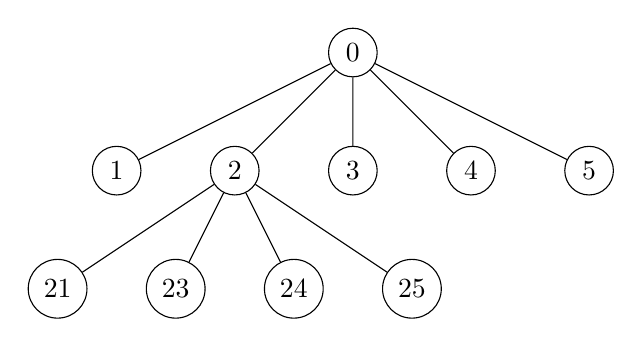
\begin{tikzpicture}[every node/.style={draw,circle}]
  \node (0) {0}
  child {node(1) {1}}
  child {node(2) {2}
    child {node(21) {21}}
    child {node(23) {23}}
    child {node(24) {24}}
    child {node(25) {25}}
  }
  child {node(3) {3}}
  child {node(4) {4}}
  child {node(5) {5}};
\end{tikzpicture}

The number of keys stored in each node will be increased exponentially
as $n - k$ becomes big. Up to $(7,10)$ threshold seems practical.

\subsubsection*{DSA, ECDSA}
BFTKV implements a DSS threshold scheme introduced by Gennaro et
al.\ \cite{Gennaro}.
Since the scheme has a restriction such as $n \geq 2t$ in the $(t,
n)$-threshold scheme, we no longer be able to use the quorum threshold
for $(t, n)$, but we follow the protocols between the client and a
quorum. The signing protocol consists of three phases:
\begin{enumerate}
\item Collect joint shared secrets generated by each quorum member:
  $\{(i, f_j(i)) | f_j(0) = k_j\}_{\{i = 1 \dots n, j \in Q\}}$
\item Distribute the secrets to the quorum and calculate
  $r=g^{k^{-1}} \bmod p \bmod q$ where $k$ is the
  joint Shamir's shared secret (i.e., $k = \sum k_i$)
\item Distribute r to the quorum and calculate $s=k(m+xr) \bmod q$
  from each $s_i=k_i(m+x_ir) \bmod q$ returned from each quorum member
\end{enumerate}


\section{Security Analysis}
We look into attacks against the fundamental property:
$READ(Q_1,x) = READ(Q_2,x)$ for $\forall Q_1, Q_2 \in QS$, which is
known as equivocation.  The best that attackers can do is divide a
clique into two sets and ask each set to sign $\langle x,t,v \rangle$
and $\langle x,t,v' \rangle$ separately. Then do the {\em write}
protocol for the target nodes with collected signature sets $S$ and
$S'$. Honest servers will refuse the request because it does not
satisfy the basic $b$-masking quorum condition: $|S| \geq b+1$. But
with $b+1$ colluding nodes, the attack will succeed.

\newcommand{\slice}[4]{
  \pgfmathparse{0.5*#1+0.5*#2}
  \let\midangle\pgfmathresult

  % slice
  \draw[thick,fill=black!10] (0,0) -- (#1:1) arc (#1:#2:1) -- cycle;

  % outer label
  \node[label=\midangle:#4] at (\midangle:1) {};

  % inner label
  \pgfmathparse{min((#2-#1-10)/110*(-0.3),0)}
  \let\temp\pgfmathresult
  \pgfmathparse{max(\temp,-0.5) + 0.8}
  \let\innerpos\pgfmathresult
  \node at (\midangle:\innerpos) {#3};
}

\begin{tikzpicture}[scale=1.5]

\newcounter{a}
\newcounter{b}
\foreach \p/\t/\l in {25//,40/$\mathcal{H}_1$/Honest nodes,
20/$\mathcal{F}$/Faulty nodes, 40/$\mathcal{H}_2$/Honest nodes}
  {
    \setcounter{a}{\value{b}}
    \addtocounter{b}{\p}
    \slice{\thea/100*360}
          {\theb/100*360}
          {\t}{\l}
  }

\end{tikzpicture}


The maximum number of signatures dishonest clients can get is
$b+(n-b)/2$. Therefore, to overcome the attack we need
\[ n-b > b+(n-b)/2 \Rightarrow n > 3b \]

\subsubsection*{Detecting equivocation on read}
Even if the number of faulty nodes exceeds the above threshold, the
system can detect malicious actions with the following probability
\begin{align*}
  F_p &= Pr[Q \cap \mathcal{H}_1 \neq \emptyset \wedge Q \cap
        \mathcal{H}_2 \neq \emptyset] \\
      & = 1 - Pr[Q \subseteq \mathcal{F} \cup \mathcal{H}_1] \\
      & = 1 - ((n + f) / 2n)^{|Q|}
\end{align*}
when $f > b$ and $|Q| < (f + n)/2$, where $f = |\mathcal{F}|$ is the
number of the faulty nodes, assuming the sizes of $\mathcal{H}_1$ and
$\mathcal{H}_2$ are the same.

In the case of $f \le b$ the detection rate is always 100\% because it is
guaranteed that clients can always find a valid value and anything
other than that is the result of malicious actions. When the number of
faulty nodes exceeds the threshold, i.e., $f > b$, it will be possible that
the client cannot detect all malicious actions. Since the minimum
quorum size is $(n-1)/3$ it does not need to consider the case where
$|Q| < n/3$. Also, if the size exceeds $(f+n)/2$ any quorum always
includes at least one node from each $\mathcal{H}_i$ which makes the
detection rate 100\%.

\ifdefined\ABSTRACT
\else
\begin{tikzpicture}[xscale=6,yscale=6]
  \draw [<->] (0,0.9) -- (0,0) -- (1.0,0);
  \node [below right] at (1,0) {$|Q|$};
  \node [left] at (0,{1-pow(17/300,0.7)}) {$1$};
  \node [left] at (0,0) {$0$};
  \node [below] at (0.3,0) {$n/3$};
  \node [below] at (0.7,0) {$(f+n)/2$};
  \draw[dashed, domain=0:0.3] plot (\x, {1-pow(17/300,\x)});
  \draw[thick, domain=0.3:0.7] plot (\x, {1-pow(17/300,\x)});
  \draw[dashed, domain=0.7:1.0] plot (\x, {1-pow(17/300,0.7)});
\end{tikzpicture}
\fi

For example, assume we choose a quorum $|Q| = 3b+1$ out of $n = 4b+1$,
which is the default setup of the kv quorum system, the detection rate
is 100\% up to $f = 2b$ failure nodes.

\ifdefined\ABSTRACT
\else
\begin{tikzpicture}[xscale=6,yscale=6]
  \draw [<->] (0,1.05) -- (0,0) -- (1.05,0);
  \node [left] at (0,1) {$1$};
  \node [left] at (0,0) {$0$};
  \node [below] at (0.3,0) {$n/3$};
  \node [below] at (0.7,0) {$2n/3$};
  \node [below] at (1,0) {$n$};
  \node [right] at (1.05,0) {$f$};
  \draw[thick, smooth] (0,1) to (0.6,1) to [out=0,in=90] (1,0);
\end{tikzpicture}
\fi


\ifdefined\ABSTRACT
\section{Conclusions}
\else
\section{Conclusions and Future Work}
\fi
We developed an efficient and secure distributed key-value store which
can be an answer for a long standing problem: How to authenticate
public keys without relying on central authorities. With BFTKV,
users no longer need to confirm peers' fingerprints or to scan a QR
code in person to ``authenticate'' the public key, which is the ways
most secure chat apps do at the moment. For example, see ``Security
considerations'' from Signal protocols which is one of the most
acclaimed peer-to-peer secure protocols \cite{signal}.
The graph driven architecture gives flexibility to the system, which
makes it possible to join / leave freely without any additional
authorization mechanism. This property makes the system transparent to
anyone, which is especially important for end-to-end systems where we
do not trust any entity even if it is the one who is running the
application systems.

Unlike most other key-value stores, BFTKV provides strong encryption
and signature schemes with a threshold cryptosystem as well. With
these features and the robust and open key-value storage, the system
will be an ideal platform to build blockchain technologies.

Also with the unique threshold password authentication system, it
solves problems like recovering from a key-loss situation and
supporting multiple devices under the same user ID. Most permissioned
systems will suffer these nasty problems when they actually deploy a
system. BFTKV integrates all those features into a Byzantine
fault-tolerant distributed key-value store.

\ifdefined\ABSTRACT
\else
\subsecion*{Future Work}
Scalability of bitcoin blockchain is excellent -- you can add as many
nodes as you want and it will not affect the whole system, but the
latency and throughput of the whole process is terrible -- it takes
one hour to settle a transaction.
On the other hand, BFT type of blockchain settles transactions in a
range from sub milliseconds to a few seconds, but scaling out is
difficult. Specifically, with quorum systems we have theoretical lower
bounds such as $n = 3f + 1$ and we cannot do anything about it.

BFTKV can separate the role of the node into two parts: signing and
reading / writing, corresponding to the auth quorum and kv quorum for
load balancing.
Once a transaction gets a collective signature, the transaction
can be stored in any way. The only concern is how to know a
transaction is latest. Each transaction has the timestamp and we can
easily get the latest $\langle x, t, v \rangle$ corresponding to a $x$
in a node but we do not know if other nodes might have a newer
value. BFTKV addresses this issue by a simple quorum system, i.e., as
long as $\forall Q_1, Q_2 \in QS, |Q_1 \cap Q_2| > f$ holds, at least
one node in a quorum has the latest value and the client will choose
that one. This method is simple but it is difficult to scale out. We
need to collect data from at least $f+1$ nodes, which depends on the
total number of servers.

Another concern is the number of collective signatures. Increasing the
number of servers does not help improve the throughput at all, because
every available server in quorum cliques needs to get invovled in
the signing process. Also it will increase the number of the
collective signatures so that each client and kv node needs to verify
more signatures.
One of the ideas to address this issue is to use a threshold signature
to combine the set of collective signatures so that each node verifies
the signature only once. But we need a dealer for the threshold
signature scheme and it will contradict the decentralized concept and
make the system less flexible.
\fi


\begin{thebibliography}{99}

\bibitem{bitcoin}
  Nakamoto, S. (2008) Bitcoin: A Peer-to-Peer Electronic Cash System

\bibitem{Delhi:1}
  Malhi, D. and Reiter, M. (1998). Byzantine Quorum Systems

\bibitem{Delhi:2}
  Malhi, D. and Reiter, M. (1998). Secure and Scalable Replication in Phalanx

\bibitem{Gennaro}
  Gennaro, R., Jarecki, S., Krawczyk, H. and Rabin, T. (1999). Robust
  Threshold DSS Signatures

\bibitem{shoup}
  Shoup, V. Practical Threshold Signatures
  
\bibitem{shamir}
  Shamir, A. (1979) How to Share a Secret

\bibitem{garay}
  Garay, J. A., Gennarob, R., Jutlab, C., Rabin, T. (2000)  Secure
  distributed storage and retrieval

\bibitem{rabin}
  Rabin, T. (1998) A Simplified Approach to Threshold and Proactive RSA

\end{thebibliography}


\section*{Acknowledgements}
We would like to thank Prof.~Idit Keidar for her expert advices about
the quorum systems. In fact, the idea of separating the KV quorum
system from the auth quorum system first appears in her email
messages. Also Dr.~Edward Bortnikov and Prof.~Juan A.~Garay helped us
move the project forward in many ways.


\newpage
\section*{Algorithms}
%
% algorithms
%
\begin{algorithm}
  \caption{GetQC}
  \SetAlgoNoLine
  \KwIn{$G$: a graph, $s$: the start node, $L$: the maximum distance}
  $queue \leftarrow {(s, 0)}$\;
  $QC = \{\}$\;
  \Repeat{$queue = \{\}$}
  {
    $(v, d) \leftarrow dequeue()$\;
    \If{$d \ge L$}{break}
    $QC = QC \cup \text{FindMaximalClique}(v)$\;
    \For{each node $n \in v.adj$}
    {
      enqueue($n, d + 1$) if $n$ has not been visited\;
    }
  }
  Check if $\forall C_1, C_2 \in QC, C_1 \cap C_2 = \emptyset$\;
  return $QC$
\end{algorithm}

\begin{algorithm}
  \caption{FindMaximalClique}
  \SetAlgoNoLine
  \KwIn{$G$: a graph, $s$: the start node}
  $C \leftarrow {s}$\;
  \For{$v \in G.V$}
  {
    $C = C + {v} \text{ if } (c_i, v) \text{ and } (v, c_i)
    \text{ for } \forall c_i \in C$\;
  }
  \If{$|C| < 4$}{return $\bot$}
  return $C$
\end{algorithm}

\begin{algorithm}
  \caption{Verification of Signature Sets}
  \SetAlgoNoLine
  \KwIn{$S = \{S_i\}, S_i = Sign_{Q_i}(\langle x, t, v, s_C \rangle)$}
  $Cliques = FindMaximalCliques(self)$\;
  \For{$clique \in Cliques$}
  {
    \If{not $VerifySS(clique, S)$}
    {
      return $False$\;
    }
  }
  return $True$\;
\end{algorithm}

\begin{algorithm}
  \caption{Verification of Quorum Certifiate}
  \SetAlgoNoLine
  \KwIn{Cert}
  $Clique = FindMaximalClique(self)$\;
  $Counter = 0$\;
  \For{each $c \in $ Cert}
  {
    \If{$c.Issuer \in Clique$ {\bf and} $Verify(c.Issuer,
      c.Signature)$
    }{
      $Counter$++\;
    }
  }
  \eIf{$Counter > 2 \cdot |Clique| / 3$}
  {
    return $True$\;
  }{
    return $False$\;
  }
\end{algorithm}

\begin{algorithm}
  \caption{Equivocation Check}
  \SetAlgoNoLine
  \KwIn{$req = \langle x, t, v, s_C, S \rangle$}
  $z = Store[x, t]$\;
  \If{$z \neq \bot$ {\bf and} $req.v \neq z.v$}
  {
    $Revoke(req.S \cap z.S)$\;
  }
\end{algorithm}

\begin{algorithm}
  \caption{TOFU enforcement}
  \SetAlgoNoLine
  \KwIn{$req = \langle x, t, v, s_C, S \rangle$}
  Verify $req.s_C$ with quorum certificate\;
  \eIf{$Store[x, 0] = \bot$\;
  }{
    $Store[x, t] = req$\;
  }{
    $last = Store[x, t-1]$\;
    \eIf{$last.s_C.cert.ID$ = $req.s_C.cert.ID$\;
    }{
      $Store[x, t] = req$\;
    }{
      Error\;
    }
  }
\end{algorithm}

\ifdefined\ABSTRACT
\else

\begin{algorithm}
  \caption{Join}
  \SetAlgoNoLine
  \KwIn{Cert}
  $G.V = Cert.sigs[*].cert$\;
  $peers = G.V$\;
  \For{$peers = \bot$}
  {
    $newPeers = \{\}$\;
    \For{$peer \in peers$}
    {
      Send $Cert$ to $peer.addr$\;
      $certs = $ Receive()\;
      $newPeers = newPeers \cup (certs \setminus G.V$)\;
      $G.V = G.V \cup certs$\;
    }
    $peers = newPeers$\;
  }
\end{algorithm}

\begin{algorithm}
  \caption{Register}
  \SetAlgoNoLine
  \KwIn{$req$: a client certificate, $proof$: the proof of the password
    authentication}
  $found$ = $Store[req.x]$\;
  \If{$found \neq \bot$ {\bf and} $req.s_C.ID = found.s_C.ID$}
  {
    $clique = FindMaximalClique(self)$\;
    \If{$proof \subseteq clique$ {\bf and} $|proof| \ge
      |clique|\cdot2/3$}
    {
      $Sign(req)$\;
    }
  }
\end{algorithm}

\fi


\end{document}
